
\documentclass[11pt]{report}
\usepackage{geometry}
\geometry{letterpaper}

%-----------------------------------

%---------------------------------------------
\setlength{\textheight}{630pt}
\setlength{\textwidth}{450pt}
\setlength{\oddsidemargin}{14pt}
\setlength{\parskip}{1ex plus 0.5ex minus 0.2ex}


%----------------------------------------
\usepackage{amsmath}
\usepackage{layout}
\usepackage{color}
\usepackage{array}
\usepackage{bm}
\usepackage{graphicx}
\usepackage{longtable}
%
\usepackage[comma,numbers,sort,compress]{natbib} % numbered, sequential refs 
\renewcommand{\bibsection}{\subsection{\bibname}} %  makes bib a numbered subsection 
\renewcommand{\bibname}{References} % use References not Bibliography for section name
%----------------------------------------------

\usepackage[us,12hr]{datetime}
\usepackage{fancyhdr} \pagestyle{fancy}
\setlength\headheight{15pt}
\lhead{\small{User's Guide - \textit{WARP3D}}}
\rhead{\small{Material: \textit{crystal plasticity}}}
\fancyfoot[L] {\small{\  Updated:  \today\ at \currenttime}}

%\fancyfoot[L] {\small{\textit{Chapter {\thechapter}}\ \   (Updated: 8-10-2015. 9:00 AM)}}
\fancyfoot[C] {\small{\thesection-\thepage}}
\fancyfoot[R] {\small{\textit{Elements and Material Models}}}

%---------------------------------------------------
\usepackage{graphicx}
% \usepackage[labelformat=empty]{caption}
\numberwithin{equation}{section}

%---------------------------------------------
%     --- make section headers in helvetica ---
%
\usepackage{sectsty} 
\usepackage{xspace}
\allsectionsfont{\sffamily} 
\sectionfont{\large}
\usepackage[small,compact]{titlesec} % reduce white space around sections
%---------------------------------------------->
%
%
%   which fonts system for text and equations. with all commented,
%   the default LaTex CM fonts are used
%
%
\frenchspacing
%\usepackage{pxfonts}  % Palatino text 
%\usepackage{mathpazo} % Palatino text
%\usepackage{txfonts}
\usepackage[stable]{footmisc}

%---------  local commands ---------------------

\newcommand{\ttt} {\texttt}  %typewriter text
\newcommand{\tb} {\textbf}
\newcommand{\nf} {\normalfont}
\newcommand{\df} {\dotfill}
\newcommand{\nin} {\noindent}
\newcommand{\bmf } {\boldsymbol }  %bold math symbol
\newcommand{\bsf } [1]{\textrm{\textit{#1}}\xspace}
\newcommand{\ul} {\underline}
\newcommand{\hv} {\mathsf}   %helvetica text inside an equation
\newcommand{\eg}{\emph{e.g.},\xspace}
\newcommand{\ie}{\emph{i.e.},\xspace}
\newcommand{\ti}{\emph}
\newcommand{\bardelta}{\bar \delta}
\newcommand{\barDelta}{\bar \Delta}
\newcommand{\veps}{\varepsilon}
\newcommand{\noi}{\noindent}

\newenvironment{offsetpar}[1]%
{\begin{list}{}%
         {\setlength{\leftmargin}{#1}}%
         \item[]%
}
{\end{list}}

%
%
%        optional definition for bullet lists which
%        reduces white space.
%
\newcommand{\squishlist}{
 \begin{list}{$\bullet$}
  { \setlength{\itemsep}{0pt}
     \setlength{\parsep}{3pt}
     \setlength{\topsep}{3pt}
     \setlength{\partopsep}{0pt}
     \setlength{\leftmargin}{1.5em}
     \setlength{\labelwidth}{1em}
     \setlength{\labelsep}{0.5em} } }

\newcommand{\squishlisttwo}{
 \begin{list}{$\bullet$}
  { \setlength{\itemsep}{0pt}
     \setlength{\parsep}{0pt}
    \setlength{\topsep}{0pt}
    \setlength{\partopsep}{0pt}
    \setlength{\leftmargin}{2em}
    \setlength{\labelwidth}{1.5em}
    \setlength{\labelsep}{0.5em} } }

\newcommand{\squishend}{
  \end{list}  }
%


%-------------------------------------
\newcounter{sectrefs}
\setcounter{sectrefs}{0}
\setcounter{chapter}{3}
\setcounter{section}{11}
\setcounter{figure}{0}
\renewcommand{\thefigure}{\thesection.\arabic{figure}}
%
%--------------------------------------
%
%
%		Editing
\newcommand{\medit}{\color{blue}}
\newcommand{\eedit}{\color{black}}
\definecolor{gold}{rgb}{0.83, 0.69, 0.22}
%
%
%              start document 
%              ==========
%
%
\begin{document}

\section{Material Model Type: \textit{cp}\footnote{The CP model was developed and implemented in WARP3D by Dr. 
Mark Messner \cite{MMthesis14} in the course of his PhD studies. Professor
Armand Beaudoin (U-Illinois) provided invaluable guidance in development of the 
formulation and code.}}
Constitutive models formulated using the concepts of crystal plasticity (CP) aim to capture the response 
of deformation in crystals and polycrystals by representing the composition of  shear deformations along each 
discrete, crystallographic slip system.  CP models serve to describe the collective motion of dislocations 
in a manner suitable for finite element simulations \cite{ REHTBR10,BA13}. The core feature set of a CP 
model is the variety of relationships provided to couple the shear strain rate to shear stress on the slip 
directions for each slip system of the crystal lattice. The CP implementation consists of a description of 
kinematics and a (local) constitutive relation for slip system response, \eg mechanical threshold stress. 
The CP material in WARP3D provides a selection of constitutive relations to link shear strain rates and 
stresses on slip planes. Moreover, the code is designed to simplify greatly the inclusion of new models 
at this scale. At present, the
CP model supports standard FCC and BCC lattice systems with 12 slip systems, the expanded 48 slip systems for BCC, and a single slip plane (010)/direction [100]
which may prove useful.
Additional lattice systems may be added readily by research-oriented users.
Starting from the scale of the crystal lattice, generation of the continuum representation at 
Gauss points (Cauchy stress tensors, deformation rate tensors and material tangents for 
implicit global frameworks), involves considerable complexity (mainly geometry) to support 
a global large-rotation, finite-strain simulation.  Finite element codes accomplish this process 
following a variety of routes dictated by their overall framework to incorporate large rotations 
and finite strains at the continuum scale. The present CP implementation embodies a rigorous 
formulation derived to provide consistency with the Green-Naghdi (unrotated) deformation  
rates and Cauchy stresses adopted for constitutive modeling in WARP3D (described in Chapter 1).

Crystal plasticity models thus differ from the typical continuum material models available in 
WARP3D in that two distinct types of parameters define the material  properties. The first type 
includes the  elastic constants,
flow properties for slip systems, thermal expansion coefficients, etc.  The second type 
comprises a set of (3) Euler angles defining  initial orientation of the atomic (crystal) 
lattice relative to the (global) model coordinate system.

Depending on the goals of a simulation, CP models may be employed at  differing length-scales. For example: 

\small
\squishlist
\item Each grain (or possibly a collection of identical grains) is represented by multiple 
(often many) finite elements to capture spatial gradients of displacement, strain and 
stress fields over the grains. All elements in a grain have the same crystallographic 
properties (lattice structure, elastic constants, thermal constants, slip  hardening behavior, etc.) 
and orientation of the slip planes relative to the model coordinate system. 
Adjacent grains generally (but are not required to) 
have the same crystallographic properties but different orientations of the slip planes. 
A solution with this approach enforces compatibility of 
deformation within grains via shared nodal displacements and displacement 
compatible element formulations. Stress equilibrium within grains is 
enforced weakly through the usual Galerkin weak form of displacement based 
finite element formulations.
\item
Individual grains are not modeled. Rather, each finite element represents a 
geometrically larger region of a polycrystalline material containing an aggregate of 
grains with differing crystallographic properties/orientations. Element sizes have 
sufficient scale for practical modeling of physical components or systems. Users may 
assign multiple crystals (properties and/or orientations) to finite elements.
The homogenized behavior of the polycrystalline material is achieved through a Taylor \cite{T38} 
approximation which enforces identical strain increments (rates) in each material at the 
Gauss point. The resulting (not necessarily equilibrium) stresses are averaged. 
This approach creates a simple reduced, multi-scale model. A single finite element on 
the scale of centimeters can represent an polycrystal with a length-scale on the order of microns.
\squishend
\normalsize
 To facilitate the various types of simulations anticipated to use the CP material model, 
 the input of properties is separated into three parts: (1) the crystal elastic and flow 
 properties \ie a crystal \ti{type} is defined and identified by an integer value, (2) the 
 lattice orientations relative to the model (global system), and (3) other values 
 including the thermal expansion coefficient, mass density,  tolerances for iterative 
 algorithms in the CP routines, etc. The end result in each case is a named \ti{material} 
 in the WARP3D scheme for assignment of material information to finite elements. 
 Numbers of  such named materials may be defined as required to meet the complexity 
 of representing the construction of a
 component. Materials other than the CP model available in
 WARP3D may be defined and associated with other finite elements
 in the mesh. The options to define a \ti{material} for association with finite elements 
 are summarized briefly here to illustrate the modeling capabilities with details 
 provided later in this section.
 
 
 \small
\squishlist
%
\item One or more \ti{crystals} numbered 1, 2, 3, $\dots$  are defined. Provided 
information includes the lattice structure (fcc, bcc, single $\dots$), type of elasticity, 
selection of the slip strain rate-shear stress flow model and values of associated parameters.
%
\item One or more named \ti{materials}, \eg  $\hv{AlLi2099, 
Gr91, T92, ...}$ is defined each
making reference to a single crystal (by number) and having a single orientation. This 
approach works well when material specification
for a simulation model requires only a few crystals and/or orientations.
Input for the named material includes the crystal number, one set of (3) orientation 
angles, thermal properties, mass density, tolerances for internal CP computations. 
Each named material may be then associated
with any number of finite elements via the usual input commands employed for 
all other material models in WARP3D (see Section 2.3), \eg \ttt{elements} 
\ttt{2000-10000 type l3disop} \ttt{nonlinear  material Gr91 bbar center\_output}$\ \dots $
%
\item The next approach proves more suitable for models where only a few crystals 
but many different orientations are needed. Each finite element is assigned 
a single crystal and a single lattice orientation. The named material now provides the
crystal number but the 3 orientation angles 
are replaced by the 
name of a flat (text) file; this file lists finite element numbers and the 
three Euler angles (one line per element).
%
\item In the most general scheme, polycrystal homogenization
 (via the Taylor approximation) is achieved 
through a flat text file with each line containing: an element number, a crystal 
number and 3 Euler angles. Each line thus associates
a crystal number and orientation angles with an element. Multiple lines
may be defined for an element listing different (or same) crystal numbers
and angles as needed to represent material properties. The number of 
lines (crystals) per element and the file name are specified in 
properties of the named material. This approach 
provides considerable flexibility to define complex and spatially
varying material properties
throughout the model.
%
\squishend
\normalsize

 
 
\noi This section continues with a brief summary of key features of the CP formulation within the
WARP3D  framework for implicit solutions including large rotations and finite strains. The
CP model formulation draws heavily on the concepts described in \cite{KBT02,ABB03}. Appendix J
provides full details of the 
formulation and numerical algorithms. Here, the description focuses 
on specification for the crystal properties, orientations and model output.



\subsection{Kinematics}

This section summarizes key features of the kinematics for
the Green-Naghdi objective stress rate adopted as the overall framework 
for large-rotations and finite-strains in WARP3D. The material
stress rate differs in various  objective rate theories
that include plastic vorticity, \ie a material model designed for a
Jaumann rate becomes kinematically incorrect in a solution framework
that uses the Green-Naghdi rate and vice-versa. An interesting observation
emerges from a rigorous derivation: stress integration for crystal plasticity
requires either the macroscale, total vorticity or the microscale
plastic vorticity, but does not require both.

\begin{figure}
\begin{centering}
\includegraphics{coordinates}
\par\end{centering}

\caption{
\small 
Coordinate systems for the crystal plasticity kinematic framework.
Integration of the objective stress rate occurs in the unrotated (intermediate)
configuration. The kinematics of crystal plasticity are defined in
the lattice coordinates. \label{fig:coords}
\normalsize}
\end{figure}


Figure \ref{fig:coords} shows the kinematic framework. Stress integration
with the Green-Naghdi rate takes place in the unrotated intermediate
or corotational frame -- the remainder of the configurations are standard
for crystal plasticity kinematics. The corotational frame
follows from a polar decomposition of the total deformation gradient
$\mathbf{F}$ into a total rotation and a total stretch:

\begin{equation}
\mathbf{F}=\mathbf{R}\mathbf{U}\ .\label{eq:polar}
\end{equation}
A multiplicative decomposition of the deformation gradient yields
$\ensuremath{\mathbf{F}=\mathbf{F}^{e}\mathbf{F}^{p}=\mathbf{V}^{e}
\mathbf{R}^{e}\mathbf{R}^{p}\mathbf{U}^{p}}$,
which decomposes both the elastic and plastic deformations into an
associated stretch and rotation. For the moment, neglect the elastic
stretch $\mathbf{V}^{e}$, then
\[
\ensuremath{\mathbf{F}=\mathbf{R}^{e}\mathbf{R}^{p}\mathbf{U}^{p}.}
\]
The small-strain nature of metal elasticity justifies this assumption.
On comparing this expression to the polar decomposition of the total
deformation gradient in Eq. \ref{eq:polar}, we have:
\[
\mathbf{R}=\mathbf{R}^{e}\mathbf{R}^{p}.
\]
After substituting and rearranging $\mathbf{F}=\mathbf{R}\mathbf{U}^{p}$.
The elastic stretch is now re-introduced as a small deviation from
the identity tensor such that $\mathbf{V}^{e}=\mathbf{I}+\bm{\varepsilon}$.
The final decomposition of the deformation gradient becomes:
\[
\mathbf{F}=\left(\mathbf{I}+\bm{\varepsilon}\right)\mathbf{R}\mathbf{U}^{p}
\]
The top part of Fig. \ref{fig:coords} shows the three coordinate
systems defined by this decomposition of the deformation gradient.

After eliminating quadratic terms in $\bm{\varepsilon}$ and $\dot{\bm{\varepsilon}}$,
the spatial velocity gradient becomes:
\[
\mathbf{L}=\dot{\mathbf{F}}\mathbf{F}^{-1}=\dot{\mathbf{R}}\mathbf{R}^{T}+
\dot{\bm{\varepsilon}}+\dot{\mathbf{R}}\mathbf{R}^{T}\bm{\varepsilon}-\bm{\varepsilon}
\dot{\mathbf{R}}\mathbf{R}^{T}+\mathbf{R}\bar{\mathbf{l}}^{p}\mathbf{R}^{T}+
\bm{\varepsilon}\mathbf{R}\bar{\mathbf{l}}^{p}\mathbf{R}^{T}-
\mathbf{R}\bar{\mathbf{l}}^{p}\mathbf{R}^{T}\bm{\varepsilon}.
\]
In this equation $\bar{\mathbf{l}}^{p}=\dot{\mathbf{F}}^{p}\mathbf{F}^{p-1}$
defines a constitutive tensor; kinematically, this is the plastic
velocity gradient pulled back to the corotational, intermediate frame.
The symmetric and skew parts of this expression are:

\begin{equation}
\mathbf{D}=\frac{1}{2}\left(\mathbf{L}+\mathbf{L}^{T}\right)=
\dot{\bm{\varepsilon}}+\bm{\varepsilon}\bm{\Omega}-\bm{\Omega}\bm{\varepsilon}+
\mathbf{R}\bar{\mathbf{d}}^{p}\mathbf{R}^{T}+
\bm{\varepsilon}\mathbf{R}\bar{\mathbf{w}}^{p}\mathbf{R}^{T}-
\mathbf{R}\bar{\mathbf{w}}^{p}\mathbf{R}^{T}\bm{\varepsilon}\label{eq:D}
\end{equation}

\begin{equation}
\mathbf{W}=\frac{1}{2}\left(\mathbf{L}-\mathbf{L}^{T}\right)=
\bm{\Omega}+\mathbf{R}\bar{\mathbf{w}}^{p}\mathbf{R}^{T}+
\bm{\varepsilon}\mathbf{R}\bar{\mathbf{d}}^{p}\mathbf{R}^{T}-
\mathbf{R}\bar{\mathbf{d}}^{p}\mathbf{R}^{T}\bm{\varepsilon}.\label{eq:W}
\end{equation}

\noi Here, $\bar{\mathbf{d}}^{p}$ is the symmetric part of $\bar{\mathbf{l}}^{p}$,
$\bar{\mathbf{w}}^{p}$ is the skew part, and $\bm{\Omega}=\dot{\mathbf{R}}\mathbf{R}^{T}$
denotes the total spin. The skew part of $\bar{\mathbf{l}}^{p}$ (the
plastic vorticity $\bar{\mathbf{w}}^{p}$ is not equal, in general,
to the plastic spin $\dot{\mathbf{R}^{p}}\mathbf{R}^{pT}$. There
is no kinematic reason to neglect either the spin or the vorticity.
To make Eq. \ref{eq:D} into a stress rate, we adopt the usual assumption
of small elastic strains and apply the elasticity tensor $\mathbf{C}$
such that $\mathbf{C}:\dot{\bm{\varepsilon}}=\dot{\bm{\sigma}}$:

\begin{equation}
\mathbf{C}:\mathbf{D}=\dot{\bm{\sigma}}+\bm{\sigma}\bm{\Omega}-
\bm{\Omega}\bm{\sigma}+\mathbf{C}:\left(\mathbf{R}\bar{\mathbf{d}}^{p}\mathbf{R}^{T}\right)+
\bm{\sigma}\mathbf{R}\bar{\mathbf{w}}^{p}\mathbf{R}^{T}-
\mathbf{R}\bar{\mathbf{w}}^{p}\mathbf{R}^{T}\bm{\sigma}\label{eq:pre-gn}
\end{equation}

\begin{equation}
\check{\bm{\sigma}}=
\mathbf{C}:\left(\mathbf{D}-\mathbf{R}\bar{\mathbf{d}}^{p}\mathbf{R}^{T}\right)-
\bm{\sigma}\mathbf{R}\bar{\mathbf{w}}^{p}\mathbf{R}^{T}+
\mathbf{R}\bar{\mathbf{w}}^{p}\mathbf{R}^{T}\bm{\sigma}=\dot{\bm{\sigma}}+
\bm{\sigma}\bm{\Omega}-\bm{\Omega}\bm{\sigma}.\label{eq:GN-expand}
\end{equation}

This $\check{\bm{\sigma}}$ is the Green-Naghdi objective stress rate. 
The material stress rate for a computational framework
using the Green-Naghdi rate becomes:
\[
\check{\bm{\sigma}}=
\mathbf{C}:\left(\mathbf{D}-\mathbf{R}\bar{\mathbf{d}}^{p}\mathbf{R}^{T}-
\bm{\varepsilon}\mathbf{R}\bar{\mathbf{w}}^{p}\mathbf{R}^{T}+
\mathbf{R}\bar{\mathbf{w}}^{p}\mathbf{R}^{T}\bm{\varepsilon}\right).
\]
In the absence of plastic spin ($\bar{\mathbf{w}}^{p}$), the stress rate
becomes the usual rate form for conventional
plasticity models (discussed in Chapter 1). As observed above, the Green-Naghdi
rate has a correction term to include effects of plastic spin:
\[
\check{\bm{\sigma}}^{corr}=\mathbf{C}:\left(-\bm{\varepsilon}\mathbf{R}
\bar{\mathbf{w}}^{p}\mathbf{R}^{T}+
\mathbf{R}\bar{\mathbf{w}}^{p}\mathbf{R}^{T}\bm{\varepsilon}\right).
\]
The Green-Naghdi rate does not require the macroscopic vorticity
W but does require the microscopic plastic vorticity $\bar{\mathbf{w}}^{p}$.
This results holds after
effects of lattice evolution are included in the plastic constitutive
tensor $\bar{\mathbf{l}}^{p}$ (see below).

With this choice of stress
rate, the stress integration simplifies considerably once stated in
the corotational frame. A pull-back of Eq. \ref{eq:GN-expand} to
the corotational frame yields:

\begin{equation}
\dot{\mathbf{t}}=\mathbf{C}_{0}:\left(\mathbf{d}-
\bar{\mathbf{d}}^{p}\right)+\mathbf{R}\bar{\mathbf{w}}^{p}\mathbf{R}^{T}\mathbf{t}-
\mathbf{t}\mathbf{R}\bar{\mathbf{w}}^{p}\mathbf{R}^{T}\ . \label{eq:gn-warp3d}
\end{equation}

Material models in WARP3D integrate this rate of unrotated Cauchy
stress $\mathbf{t}=\mathbf{R}^{T}\bm{\sigma}\mathbf{R}$ as a function
of $\mathbf{d}$, the unrotated rate of deformation.
At this point,
the macroscale rotational response uncouples completely from the microscale
lattice rotations -- only the global rotation $\mathbf{R}$ appears.
 In one advantage of this framework, the elasticity tensor $\mathbf{C}_{0}$, may have the appropriate
form of an anisotropic tensor for the crystal system, rotated from
the initial lattice frame to the reference frame.
WARP3D handles all the rotations required for the elasticity tensor
automatically.
The user provides the appropriate anisotropic elasticity tensor
in the \emph{crystallographic frame}.
The code will provide the constant rotation into the lattice frame as well 
as the rotation into the intermediate configuration, which changes with time.
By enabling this
definition of a constant elasticity tensor in the corotational frame,
the total material rotation then updates the anisotropic elastic constants
of a crystal.
For small elastic stretches, this approach is equivalent
to elasticity models derived from a hyperelastic potential.

With Eq. \ref{eq:gn-warp3d} taken to update stresses at a material (integration)
point in a finite element, the constitutive model must then
compute the plastic deformation $\bar{\mathbf{l}}^{p}$.
For crystal
plasticity, the common kinematic assumption is an additive decomposition
of plastic shear deformations in a lattice frame \cite{A83}:

\begin{equation}
\tilde{\mathbf{l}}^{p}=
\sum_{s=1}^{n_{slip}}\dot{\gamma}^{\left(s\right)}\left(\tilde{\mathbf{b}}^{\left(s\right)}
\otimes\tilde{\mathbf{n}}^{\left(s\right)}\right)\label{eq:flow-rule}
\end{equation}

\noi where $\mathbf{b}^{\left(s\right)}$ and $\mathbf{n}^{\left(s\right)}$
denote collections of slip-system directions and normals in the lattice
frame and $\dot{\gamma}^{\left(s\right)}$ is the slip rate along
each slip system.
The geometry of the crystal system, for example
face centered cubic (FCC), defines these slip systems in the crystallographic
frame and a rigid rotation $\mathbf{g}$, calculated from the initial
grain orientations, defines the rotation between the lattice frame
and the crystallographic frame.
Finally, as Fig. \ref{fig:coords}
indicates, the model must transform this deformation tensor in the
lattice frame into the unrotated frame to specify the plastic deformation
in the corotational coordinates.
The rotation defining this transformation
is $\mathbf{R}^{p}$.
The kinematics of macroscale deformation do
not define this plastic rotation. Here, we define $\mathbf{R}^{p}$
as part of the constitutive response of the
material.
That is, the plastic rotation is part of the micro-constitutive
response, not the global kinematics.
This plastic rotation does not
affect the elasticity tensor, only the plastic rate $\tilde{\mathbf{l}}^{p}$.
This approximation appears acceptable for moderate plastic strains \cite{FS00},
where the elastic response of the material does not depend strongly
on the plastic deformation.

From these definitions, the symmetric and skew parts of plastic deformation
are:
\[
\bar{\mathbf{d}}^{p}=
\sum_{s=1}^{n_{slip}}\dot{\gamma}^{\left(s\right)}
\left(\mathbf{R}^{pT}\tilde{\mathbf{m}}^{\left(s\right)}\mathbf{R}^{p}\right)
\]
\[
\bar{\mathbf{w}}^{p}=
\sum_{s=1}^{n_{slip}}\dot{\gamma}^{\left(s\right)}
\left(\mathbf{R}^{pT}\tilde{\mathbf{q}}^{\left(s\right)}\mathbf{R}^{p}\right)
\]
with $\tilde{\mathbf{m}}^{\left(s\right)}=
\mathrm{sym}\left[\tilde{\mathbf{b}}^{\left(s\right)}\otimes\tilde{\mathbf{n}}^{\left(s\right)}\right]$
and 
$\tilde{\mathbf{q}}^{\left(s\right)}=\mathrm{skew}\left[\tilde{\mathbf{b}}^
{\left(s\right)}\otimes\tilde{\mathbf{n}}^{\left(s\right)}\right]$.
Typically the slip rate on each system is taken as power-law dependent
on a reference strain rate, the resolved shear, and a slip system
strength. \ti{Here the slip system hardening is isotropic -- all slip
systems have the same slip system strength} (this is not a limitation
of the formulation).
The slip rate relation is:

\begin{equation}
\dot{\gamma}^{\left(s\right)}=
\frac{\dot{\gamma}^{0}}{\tilde{\tau}}
\left|\frac{\tau^{\left(s\right)}}{\tilde{\tau}}\right|^{n-1}\tau^{\left(s\right)}
\label{eq:gamma-dot}
\end{equation}

\noi with $\dot{\gamma}^{0}$ a reference slip rate, $\tilde{\tau}$ the
slip system strength, and $\tau^{\left(s\right)}$ the resolved shear
on slip system $s$. 
The reference slip rate is given by $\dot\gamma^0=\dot\varepsilon$, where

\begin{equation}
\dot\varepsilon=\sqrt{ \frac{2}{3}\mathbf{D}:\mathbf{D}}=\sqrt{\frac{2}{3}\mathbf{d}:\mathbf{d}}\ ,
\label{eq:dot-gamma-0}
\end{equation}



\noi which is the macroscale strain rate.  
	This definition, together with a high value of the exponent $n$ (typically
	$n=20$) forces the material to approximate rate independent flow.
	For FCC metals, this `rate-insensitivity' is often physically appropriate
	and greatly increases the numerical stability of the material model.
	This rate insensitive flow rule can be combined with a rate dependent
	model for the full stress, where $\tilde{\tau}$ varies with the strain rate.
	With such a combination when the strain rate changes the material will
	(approximately) instantaneously achieve the new value of the flow stress,
	without any delay or overshoot caused by viscoplastic effects.


Finally, define the rate of plastic rotation:

\begin{equation}
\dot{\mathbf{R}}^{p}=\bar{\mathbf{w}}^{p}\mathbf{R}^{p}.\label{eq:rotation-update}
\end{equation}
Kinematically, this form is not rigorously correct, but it does approximate
closely the experimentally observed texture evolution in a variety
of situations (see section 5.1 in \cite{HF01}, \cite{KBA92,KBT02,MS01}).
Substitution of the macroscopic vorticity via Eq. \ref{eq:W} eliminates
the plastic vorticity from the above equation, thus making the lattice
evolution dependent only on the macroscopic vorticity and the symmetric
part of the microscopic plastic deformation.
In the presence of lattice
rotations, the formulation then continues to require only one of (1)
the macroscale, total vorticity or (2) the microscale, plastic vorticity.

\subsection{Stress Update}

A backward Euler integration of Eq. \ref{eq:gn-warp3d} defines the
stress update procedure.
To reduce computational effort an explicit
exponential integration of Eq. \ref{eq:rotation-update} provides
the plastic rotation update. Thus,

\begin{equation}
\mathbf{t}_{n+1}=
\mathbf{t}_{n}+\mathbf{C}_{0}:\left(\Delta\mathbf{d}_{n+1}-
\Delta\bar{\mathbf{d}}_{n+1}^{p}\right)+
\Delta\bar{\mathbf{W}}_{n+1}^{p}\mathbf{t}_{n+1}-
\mathbf{t}_{n+1}\Delta\bar{\mathbf{W}}_{n+1}^{p}\label{eq:stress-update-np1}
\end{equation}

\[
\Delta\bar{\mathbf{d}}_{n+1}^{p}=
\sum_{s=1}^{n_{slip}}\Delta\gamma_{n+1}^{\left(s\right)}
\left(\mathbf{R}_{n}^{pT}\tilde{\mathbf{m}}^{\left(s\right)}\mathbf{R}_{n}^{p}\right)
\]


\[
\Delta\bar{\mathbf{w}}_{n+1}^{p}=
\sum_{s=1}^{n_{slip}}\Delta\gamma_{n+1}^{\left(s\right)}
\left(\mathbf{R}_{n}^{pT}\tilde{\mathbf{q}}^{\left(s\right)}\mathbf{R}_{n}^{p}\right)
\]
\[
\Delta\bar{\mathbf{W}}_{n+1}^{p}=
\mathbf{R}_{n+1}\Delta\bar{\mathbf{w}}_{n+1}^{p}\mathbf{R}_{n+1}^{T}
\]
\[
\Delta\gamma_{n+1}^{\left(s\right)}=
\frac{\Delta\gamma_{n+1}^{0}}{\tilde{\tau}_{n+1}}
\left|\frac{\tau_{n+1}^{\left(s\right)}}{\tilde{\tau}_{n+1}}\right|^{n-1}\tau_{n+1}^{\left(s\right)}
\]

\begin{equation}
\mathbf{R}_{n+1}^{p}=\exp\left(\Delta\bar{\mathbf{w}}_{n+1}^{p}\right)\mathbf{R}_{n}^{p}.\label{eq:rotation-update-exp}
\end{equation}

These equations yield the updated stress state in the unrotated configuration
as a function of the unrotated strain increment 
$\Delta\mathbf{d}_{n+1}=\mathbf{d}_{n+1}\Delta t_{n+1}$,
the reference strain rate, and a slip-system strength (yet to be defined).
After a successful stress update, the model integrates the plastic
rotations explicitly with Eq. \ref{eq:rotation-update-exp}.
The exponential
operator ensures that successive plastic rotations remain orthogonal
transformations.
The resolved shear along a slip system should be
calculated in the current coordinates with the Cauchy stress. 
However:

\[
\tau_{n+1}^{\left(s\right)}=
\bm{\sigma}_{n+1}:\left(\mathbf{R}_{n+1}\mathbf{R}_{n}^{pT}
\tilde{\mathbf{m}}^{\left(s\right)}\mathbf{R}_{n}^{p}\mathbf{R}_{n+1}^{T}\right)=
\mathbf{t}_{n+1}:\left(\mathbf{R}_{n}^{pT}\tilde{\mathbf{m}}^{\left(s\right)}\mathbf{R}_{n}^{p}\right)
\]

\noi such that the resolved shear is also a function of the unrotated stress.

This works also assumes that the effective slip increment is the global effective
strain increment:

\begin{equation}
\Delta\gamma_{n+1}^{0}=
\sqrt{\frac{2}{3}\Delta\mathbf{D}_{n+1}:\Delta\mathbf{D}_{n+1}}=
\sqrt{\frac{2}{3}\Delta\mathbf{d}_{n+1}:\Delta\mathbf{d}_{n+1}}.\label{eq:reference-slip}
\end{equation}
\eedit

\subsection {Consistent Tangent (Symmetry/Asymmetry)}
In addition to updated Cauchy stresses at $n+1$, 
the material model routines must return the 
consistent tangent matrix for use in the global Newton iterations (all details in Appendix J).  

The non-associative  flow rule of Eq. \ref{eq:flow-rule} leads to 
a non-symmetric consistent tangent matrix.  WARP3D global solvers process both
symmetric and asymmetric systems of the linearized equilibrium
equations to support this type of formulation. Section 2.10 describes the commands to 
request a symmetric or asymmetric solver.

The asymmetric solver requires twice the memory and roughly twice the computational effort
per global Newton iteration compared to the symmetric solver. Nevertheless, the asymmetric
formulation/solver likely reduces the number of
Newton iterations for convergence sufficiently to offset the additional effort per iteration. 
The outcome of such tradeoffs proves dependent on material models, loading rates,
time step sizes, etc.

When a symmetric solver is specified, the CP model
computes an approximate, symmetrized tangent (the CP model routines are aware of the user's
selection of global equation solver).
Since this is only an approximate
tangent, the global Newton iterations may not achieve true quadratic convergence.
Users should expect the potential of additional Newton iterations per load step, 
and generally must specify 
smaller increments of load per step to achieve good convergence rates.




\subsection{Work Hardening}

The  slip-system strength, $\tilde{\tau}$,  appears in the power-law 
relations in Eqs. \ref{eq:gamma-dot}
and \ref{eq:rotation-update-exp} which link slip-strain rates to resolved shear stress.
Work hardening behavior (in FCC metals) typically follows the stages illustrated in Fig.
\ref{fig:stages-hardening}.
\begin{figure}
\begin{centering}
\includegraphics{figure_1_hardening-plot.pdf}
\par\end{centering}

\caption{\small Stages of work hardening.  The simple Voce model may
represent (one of) Stages I, II or III (with zero terminal slope). The MTS model represents Stage 
III and and optionally Stage IV.
\normalsize \label{fig:stages-hardening}} 
\end{figure} 


\noi Three options are available to describe hardening behavior through the 
evolution of $\tilde \tau$. 

\small
\squishlist
\item 
A simple temperature and rate independent Voce model
provides Stage III hardening with a zero slope in Stage IV.  By setting specific values
of the Voce model parameters, it becomes a constant linear hardening function or no hardening.
\item
A more complex Mechanical Threshold Stress \cite{FK88} hardening model, MTS, provides
temperature and rate dependent hardening in Stage III.  Stage IV has
zero slope (default) or incorporates a geometric
hardening contribution which both introduces a size effect and 
renders stage IV hardening through a local strain gradient of the elastic distortion.
\item 
A user-defined hardening function. Appendix J describes how a research-oriented user
may implement a different hardening function using the standard hardening interface 
designed into code for the CP model.
\squishend
\normalsize


\noi \textbf{Voce Hardening Function}

\noi 
A simple Voce model with no temperature or strain-rate effects is provided to model
only Stage III hardening with the form

\begin{equation}\label{eq:Voce-simple-a}
\tilde{\tau}=\tau_{y}+\tau_{w}
\end{equation}

\begin{equation}\label{eq:Voce-simple-b}
\dot{\tau}_{w}=\ensuremath{\theta_{0}\left(1-\frac{\tau_{w}}{\tau_{v}}
\right)^{m}\ \sum\limits _{s=1}^{n_{slip}}\left|\dot{\gamma}^{\left(s\right)}\right|}
\end{equation}

\noi The hardening specific  input properties (constants) are: $\tau_y, \theta_0, \tau_v, m$.
Slip system hardening is isotropic -- all slip
systems have the same slip system strength in our implementation.

Here $\tau_y$ describes the intrinsic (yield) resistance to flow, $\tau_w$
the extrinsic (hardening) resistance, and $\tau_v$ the work hardening saturation strength. 


In the general Voce form above, the Stage IV slope is zero ($\dot \tau_w \rightarrow 0$).
If desired, a constant linear hardening behavior with slope $\theta_0$ is obtained by setting
the exponent $m=0$. Similarly, an elastic-plastic behavior is obtained by setting
$\theta_0=0$. 


Use of a forward Euler integration for  $\dot{\tau}_{w}$ leads to
 
\begin{equation}\label{eq:Voce-simple-c}
\ensuremath{\tilde{\tau}_{n+1}=h_{n+1}=
\tilde{\tau}_{n}+\theta_{0}\left(1-\frac{\tilde{\tau}_{n+1}-\tau_{y}}{\tau_{v}}\right)^{m}\ 
\sum\limits _{s=1}^{n_{slip}}\left|\Delta\gamma_{n+1}^{\left(s\right)}\right|}
\end{equation}

\noi which defines the hardening function $h_{n+1}$.
No additional internal variables exist for this model.



\noi \textbf {MTS Hardening Function} 

\noi Figure \ref{fig:mts} illustrates behavior of  MTS model which
approximates both the initial strength (flow stress) of the crystal from 
inherent obstacles to dislocation motion (the
\ti{yield stress}), and the increase in strength due to forest dislocation
hardening (one common mechanism for \ti{work hardening}). The total strength (flow stress)
is written in this general form:

\begin{equation}
\tilde{\tau}=\tau_{a}+\tau_{y}\left(T,\dot{\varepsilon}\right)\frac{\mu (T)}
{\mu_{0}}+\bar \tau\left(\varepsilon_{p},T,
\dot{\varepsilon}\right)\frac{\mu (T)}{\mu_{0}}\label{eq:strength-split}
\end{equation}


 
\begin{figure}[htb]
\begin{center}
\includegraphics[trim=0.0in 3.0in 5.0in 0.2in, clip=true,scale=0.70,angle=0]{mts_figure.pdf} 
%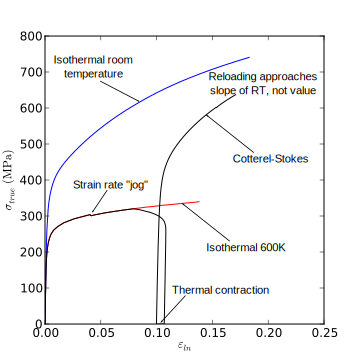
\includegraphics[scale=1.25]{cs_plot.pdf}
\caption{{\small  Behavior of the MTS hardening model.} \label{fig:mts}}
%
\end{center}
\end{figure}
%

\noindent which explicitly separates temperature and rate invariant
components of the yield stress ($\tau_a$) from scaling factors
dependent on temperature and rate ($\tau_{y}, \bar \tau$). Moreover, 
$\bar \tau$ may depend (in general) on the accumulated plastic strain ($
\sum|\gamma^{(s)}|$). The $\mu(T)/\mu_{0}$
ratio supports temperature dependent elastic properties. 



The adopted form for $\bar \tau$ is a Voce model with final Stage IV slope of zero
(modified later for geometric hardening),

\begin{equation}
\frac{d\bar{\tau}}{dt}=\theta_{0}\left ( 1-\frac{\bar{\tau}}{\tau_{v}
\left(T,\dot{\varepsilon}\right )}\right )^m \ 
\sum \limits _{s=1}^{n_{slip}}\left|\dot{\gamma}^{\left(s\right)}\right|\label{eq:mts-voce}
\end{equation}


\begin{figure}
\begin{centering}
\includegraphics{figure_2_voce-plot.pdf}
\par\end{centering} 

\caption{\small Voce law in Eq. \ref{eq:mts-voce} to define $\bar \tau$ in the MTS hardening model with exponent $m=1$ (default value of \ttt{voce\_m}). Here Stage
III has the instantaneous starting slope $\theta_{0}$ and the 
slope of Stage IV is $0$. \normalsize\label{fig:Simplified-Voce-law}}
\end{figure}


\noindent  Slip system hardening is isotropic -- all slip
systems have the same slip system strength in our implementation.
$\tau_{v}\left(T,\dot{\varepsilon}\right)$ thus defines the saturation strength
of work hardening for a given temperature and rate -- with no dependence here on
accumulated plastic strain $\veps^p$. The parameter $\theta_{0}$, with adjustment for
possible temperature dependence of the shear modulus, 
determines the initial Stage II hardening slope (see 
Figs. \ref{fig:mts}, \ref{fig:Simplified-Voce-law}).\footnote{
\ul{\textbf{The default, reference temperature in all elements is \ti{zero} in WARP3D models.}}
See Chapter 2 Section on Initial Condition for commands to set a non-zero
reference temperature. MTS hardening with temperature/rate dependencies
requires the user to consider the setting of an appropriate temperature.}

Determination of the
slip system strength ($\tilde \tau$) in Eq. \ref{eq:strength-split}
then reduces to choosing functional forms
for $\tau_{y}\left(T,\dot{\varepsilon}\right)$ and 
$\tau_{v}\left(T,\dot{\varepsilon}\right)$ and integrating the Voce expression.
Kocks, Argon and Ashby advanced the concept of the mechanical
	threshold, the flow stress at zero temperature, as a reference state for
	plastic flow \cite{KAA75}. 
	A mechanical threshold is then 
	$\hat \tau= \tau \mathrm{( 0\, K, 0\,s^{-1}) }$, 
	where $\tau = \tau \left( \dot\varepsilon,T \right)$ 
	is a kinetic law.
	In the mechanical threshold stress approach, the terms 
	$\hat\tau_{y}$ and $\hat\tau_{v}$, represent the strength 
	at 0K associated with yield and work hardening mechanisms, respectively.
	Development of the MTS model then involves adopting an Arrhenius-type 
	law to scale the mechanical threshold (strength) to a specified 
	combination of rate and temperature \cite{FK88}. 
	Applying this concept to the work hardening model
	(Eqs. \ref{eq:strength-split}
and \ref{eq:mts-voce}) we have:

\begin{equation}
\tau_{y}\left(T,\dot{\varepsilon}\right)=\hat{\tau}_{y}
\left[1-\left(\frac{kT}{\mu\left(T\right)b^{3}g_{0,y}}
\ln\frac{\dot{\varepsilon}_{0,y}}{\dot{e}}\right)^{\dfrac{1}{q_{y}}}\right]^{\dfrac{1}{p_{y}}}\ ,\label{eq:tau-y}
\end{equation}


\begin{equation}
\tau_{v}\left(T,\dot{\varepsilon}\right)=\hat{\tau}_{v}\left[1-\left(\frac{kT}{\mu\left(T\right)b^{3}g_{0,v}}\ln\frac{\dot{\varepsilon}_{0,v}}{\dot{e}}\right)^{\dfrac{1}{q_{v}}}\right]^{\dfrac{1}{p_{v}}}\ ,\label{eq:tau-v}
\end{equation}

\begin {equation}
\dot{e}=\sqrt{\frac{2}{3}\mathbf{D}:\mathbf{D}}\ .
\end{equation}

\noi where $k$ is the Boltzmann constant, $T$ is absolute temperature, $b$ is
the magnitude of the Burger's vector, $g_{0,(y,v)}$ are
normalized activation energies, $\dot{\varepsilon}_{0,(y,v)}$
are reference strain rates, and $q_{(y,v)}$, $p_{(y,v)}$
are constants related to the shape of the activation energy barrier (see expanded discussion in
Appendix J). In these equations the $(\hat{\tau}_y$, $g_{0,y}$, $\dot{\varepsilon}_{0,y}$,
$q_y$, $p_y)$, ($\hat{\tau}_v$, $g_{0,v}$, $\dot{\varepsilon}_{0,v}$,
$q_v$, and $p_v$) terms are specified input parameters.  $b$ and $k$ are the physical constants, also
specified input values and with consistent units.

The temperature dependence of shear modulus is given by

\begin{equation}
\mu\left(T\right)=\mu_{0}-\frac{D_{0}}{\exp\left({T_{0}}/{T}\right)-1}\label{eq:shear-modulus}
\end{equation}

\noindent where $\mu_{0}$, $D_{0}$, and $T_{0}$ are
all specified input parameters. 


The CP model in WARP3D implements this MTS hardening
formulation with the implicit integration (backward Euler) of Eq. \ref{eq:strength-split}.
This introduces an additional equation into the local (material) nonlinear
system of Eq. \ref{eq:stress-update-np1}, which in turn expands its linearization in Newton's method
by one row and column. The updated strength at $n+1$ is then given by
\[
\ensuremath{\tilde{\tau}_{n+1}=\tau^{a}+\left(\frac{\mu_{n+1}}{\mu_{0}}\right)\tau_{n+1}^{y}+\left(\frac{\mu_{n+1}}{\mu_{0}}\right)\tau_{n+1}^{w}}
\]
\[
\ensuremath{\tau_{n+1}^{w}=\tau_{n}^{w}+\theta_{0}\left(1-\frac{\tau_{n+1}^{w}}{\tau_{n+1}^{v}}\right)^{m}\sum\limits _{s=1}^{n_{slip}}\left|\Delta\gamma_{n+1}^{\left(s\right)}\right|}
\]
\[
\ensuremath{\tau_{n+1}^{v}=\hat{\tau}^{v}\left\{ 1-\left[\frac{kT_{n+1}}{\mu_{n+1}b^{3}g_{0}^{v}}\ln\left(\frac{\dot{\varepsilon}_{0}^{v}}{\Delta\gamma_{n+1}^{0}/\Delta t_{n+1}}\right)\right]^{1/q^{v}}\right\} ^{1/p^{v}}}
\]
\begin{equation}
\ensuremath{\tau_{n+1}^{y}=\hat{\tau}^{y}\left\{ 1-\left[\frac{kT_{n+1}}{\mu_{n+1}b^{3}g_{0}^{y}}\ln\left(\frac{\dot{\varepsilon}_{0}^{y}}{\Delta\gamma_{n+1}^{0}/\Delta t_{n+1}}\right)\right]^{1/q^{y}}\right\} ^{1/p^{y}}}\label{eq:tau_y}
\end{equation}
with:
\begin{equation}
\ensuremath{\mu_{n+1}=\mu_{0}-\frac{D_{0}}{\exp\left(\frac{T_{0}}{T_{n+1}}\right)-1}}.\label{eq:shear}
\end{equation}
These equations are combined to define the hardening function:
\begin{multline}
\ensuremath{\tilde{\tau}_{n+1}=h_{n+1}=\tau^{a}\left(1-\frac{\mu_{n+1}}{\mu_{n}}\right)+\left(\frac{\mu_{n+1}}{\mu_{0}}\right)\left(\tau_{n+1}^{y}-\tau_{n}^{y}\right)+\left(\frac{\mu_{n+1}}{\mu_{n}}\right)\tilde{\tau}_{n}+\theta_{0}\left(\frac{\mu_{n+1}}{\mu_{0}}\right)}\\
\ensuremath{\left(1-\frac{\left(\frac{\mu_{0}}{\mu_{n+1}}\right)\tilde{\tau}_{n+1}-\left(\frac{\mu_{0}}{\mu_{n+1}}\right)\tau^{a}-\tau_{n+1}^{y}}{\tau_{n+1}^{v}}\right)^{m}\ensuremath{\sum\limits _{s=1}^{n_{slip}}\left|\Delta\gamma_{n+1}^{\left(s\right)}\right|.}}
\end{multline}


\noi \ul{Stage IV Hardening}. 
Geometric hardening describes the effect on flow stress of geometrically 
necessary dislocations (GNDs) -- 
also called excess dislocations  (for early work see \cite{A70}). 
Simulations of regions with high strain gradients may benefit by  incorporating this signed 
dislocation density. For example, geometric hardening may develop
near strongly mismatched grain boundaries. The MTS model provides an option to approximate
the effect of GNDs -- those (theoretically) necessary to maintain
compatible deformation.  This signed dislocation density
contributes to the (forest) work hardening, as the accumulation of 
immobile dislocations is impacted by their geometric arrangement 
(in addition to the mean free path storage associated with the statistical 
density). Acharya \emph{et al.} \cite{ABB03}
associate these geometric dislocations with 
Stage IV hardening. Omitting some derivation and theory (see references for
details), the Nye tensor of geometrically necessary dislocations
is:

\begin{equation}
\bm{\alpha}=-\nabla\times\mathbf{F}^{e-1}
\label{eq:Nye-tensor}
\end{equation}


\noindent The density of necessary dislocations along each slip system is:

\begin{equation}
\lambda^{\left(s\right)}=\sqrt{\left(\bm{\alpha}\mathbf{n}_{s}^
{\left(s\right)}\right):\left(\bm{\alpha}\mathbf{n}_{s}^{\left(s\right)}\right)}
\label{eq:lambda-Nye}
\end{equation}

\noindent To include GND effects, Archarya \emph{et al.} suggest an addition to the Voce law
to replace Eq. \ref{eq:mts-voce}

\begin{equation}
\frac{d\bar{\tau}}{dt}=\sum\theta_{0}\left (  1-\frac{\bar{\tau}}{\tau_{v}}+
\frac{\tau_{\lambda}^{\left(s\right)}}{\bar{\tau}}\right )^m
\left|\dot{\gamma}^{\left(s\right)}\right|\label{eq:voce-with-geom}
\end{equation}

\begin{equation}
\tau_{\lambda}^{\left(s\right)}=\frac{k_{0}}{k_{1}}\,\eta\,\mu\,\lambda^{\left(s\right)}\label{eq:t-lamba}
\end{equation}


\noindent where $k_{1} = 2\,\theta_{0}/\left(\eta\,\mu(T)\,b\right)$,
$\eta=1/3$, and $k_{0}$ is a parameter (typical values
on the order of 1). Computation of the curl of the elastic deformation
through an implicit integration is cumbersome; consequently, the
computations update values of
$\tau_{\lambda}^{\left(s\right)}$ explicitly. The remainder
of the hardening evolution remains implicit, as above.

\noi \textbf {User-defined Hardening} 


\noi Design-implementation of the CP code supports user-developed, plug-in routines
to expand the options for hardening models.  The required outputs of  routines to implement
a new hardening model have  standardized parameter lists (see Appendix J for details).

To supply user-hardening parameters, WARP3D input translators scan and store the values
of crystal properties with names \ttt{u\_1, u\_2, ... u\_6}. These values are integral to data structures
for the CP model and are available to the user-hardening functions.

\begin{table}[htbp]
\small
\centering
\setlength{\extrarowheight}{3pt}

\begin{tabular}{|l|c|c|c|c|}
\hline 
\textbf{Property} & \textbf{Keyword} & \textbf{Options/type}&\textbf{Default Value}&\textbf{Units}\tabularnewline
\hline \hline
Slip system type & slip\_type & fcc, bcc, bcc48, single&fcc&--\tabularnewline \hline
Hardening model & hardening &voce&---$^\dag$&--\tabularnewline \hline
Elastic type & elastic\_type & isotropic, cubic&isotropic&--\tabularnewline \hline
Young's modulus & e & real&69000&$F/L^2$\tabularnewline \hline
Poisson's ratio & nu & real&0.33&--\tabularnewline \hline
Shear modulus (elastic) & mu & real&---$^\ddag$&$F/L^2$\tabularnewline \hline
$n$ (Eq. \ref{eq:gamma-dot}) & harden\_n & real&20&--\tabularnewline \hline
$\tau_y$ (Eq. \ref{eq:Voce-simple-a}) & tau\_y & real&0.0&$F/L^2$\tabularnewline \hline
$\tau_v$ (Eq. \ref{eq:Voce-simple-b}) & tau\_v & real&0.0&$F/L^2$\tabularnewline \hline
$m$ (Eq. \ref{eq:Voce-simple-b}) & voce\_m & real&1.0&--\tabularnewline \hline
$\theta_0$ (Eq. \ref{eq:Voce-simple-b}) & theta\_0 & real& 100&$F/L^2$\tabularnewline \hline
\end{tabular}
\caption{Crystal properties to employ the simple \ti{Voce}  hardening model. $^\dag$User must
enter the keyword $\hv{voce}$.
$^\ddag$Enter a value of  \ttt{mu} only
for the cubic anisotropy option.
\label{tab:crys-voce}}
\normalsize
\end{table}



%*******************************
\subsection{Crystal Definition}
%*******************************
A \ti{crystal} command defines a numbered $\hv{crystal}$ and
associates a set of orientation independent 
elastic, flow and hardening properties.  
Crystal numbers must start at 1 and increase sequentially, with a current limit
of 1000 such crystals.
Each phase in the material typically will be defined as different crystal.  
The
following shows an example crystal definition that invokes the
MTS hardening model with the approximate Stage IV
features for GNDs:

\small
\begin{verbatim}
  crystal 1
      properties slip_type fcc elastic_type isotropic,
      e 78810 nu 0.33,
      hardening mts harden_n 20  voce_m 1.0,
      mu_0 29630 D_0 0.0 T_0 294,
      b 3.5E-7 boltz 1.3806E-20,
      theta_0 180.0,
      tau_a 0.0,
      tau_hat_y 155.0 g_0_y 0.007808 q_y 2.0 p_y 0.5,
      eps_dot_0_y 1.0E13,
      tau_hat_v 25.0 g_0_v 0.00488 q_v 2.0 p_v 0.5,
      eps_dot_0_v 1.0E7, 
      k_0 5.0
\end{verbatim}
\normalsize

\noi Notice that all properties are listed on a single, logical line of input composed
of multiple physical lines using a comma for continuation.

\noi The key capabilities of the current crystal implementation may be described by

\small
\squishlist
\item Slip-system type: \ttt{fcc}  \{111\}$<$110$>$ [12 slip systems]; 
 \ttt{bcc} \{110\}$<$111$>$ [12 slip systems];
 \ttt{ bcc48} \{110\}$<$111$>$, \{112\}$<$111$>$, and \{123\}$<$111$>$ [48 slip systems];
    \ttt{single} -- (010) [100] 
\item Hardening model: \ttt{voce} (simple, temperature invariant), \ttt{mts}, \ttt{user}
\item Elasticity:\ttt{ isotropic}, \ttt{cubic} (anisotropy)
\squishend
\normalsize

\noi Properties of the material elasticity tensor are temperature invariant at this time,
while the plastic properties may vary with temperature in the mts hardening function.  
The elastic properties may be isotropic (property \ttt{isotropic})
or have cubic anisotropy (property \ttt{cubic}):
 \small
\squishlist
\item \ttt{isotropic}. The shear modulus for the elasticity 
tensor is computed from the specified value of $E, \nu$. 
Do not  set a value for the shear modulus (\ttt{mu}). Use property \ttt{mu\_0}
to separately set the temperature dependent reference modulus for plasticity 
computations.
\item  \ttt{cubic} anisotropy. Set the shear modulus value for the elasticity 
tensor with the property \ttt{mu}. Use property \ttt{mu\_0}
to separately set the temperature dependent reference modulus for plasticity 
computations.
 \squishend
\normalsize

\noi
For simplicity, separate Tables \ref{tab:crys-voce}, \ref{tab:crys-mts}, and
\ref{tab:crys-user}  are provided here listing the input 
properties for each of the hardening models.

Table \ref{tab:crys-voce} lists the properties for description of the simple, temperature invariant
\ti{Voce} hardening model described in Eqs. \ref{eq:Voce-simple-a} and \ref{eq:Voce-simple-b}.


Table \ref{tab:crys-mts} lists the properties for description of the general \ti{mts} hardening 
model described in Eqs. \ref{eq:Voce-simple-a} and \ref{eq:Voce-simple-b}.
If the shear modulus in the hardening equations and in the elasticity tensor both
should be constant, set \ttt{mu\_0} to the constant value and set \ttt{D\_0} = 0.


Table \ref{tab:crys-user} lists the properties for description of the  \ti{user} hardening 
model. 



\small
%\begin{table}[htb]
%\small
%\centering
\setlength{\extrarowheight}{3pt}

%\begin{tabular}{|l|c|c|c|}
\LTcapwidth=\textwidth
\begin{longtable}{|l|c|c|c|c|}
\hline 
\textbf{Property} & \textbf{Keyword} & \textbf{Options/type}&\textbf{Default Value$^\#$}&\textbf{Units}\tabularnewline
\hline \hline
Slip system type & slip\_type & fcc, bcc, bcc48, single&fcc&--\tabularnewline \hline
Hardening model & hardening & mts&--$^\dag$&--\tabularnewline \hline
Elastic type & elastic\_type & isotropic, cubic&isotropic&--\tabularnewline \hline
Young's modulus & e & real&69000&$F/L^2$\tabularnewline \hline
Poisson's ratio & nu & real&0.33&--\tabularnewline \hline
Shear modulus (elastic) & mu & real&--$^\ddag$&$F/L^2$\tabularnewline \hline
$n$ (Eq. \ref{eq:gamma-dot}) & harden\_n & real&20&--\tabularnewline \hline
$m$ (Eq. \ref{eq:mts-voce}) & voce\_m & real&1.0&--\tabularnewline \hline
Boltzmann constant & boltz & real & $1.3806\times 10^{-20}$&$F\cdot L/T$\tabularnewline \hline
Magnitude of Burgers vector & b & real&$2.86\times 10^{-7}$&L\tabularnewline \hline
$\tau_{a}$ (Eq. \ref{eq:strength-split}) & tau\_a & real&0.0&$F/L^2$\tabularnewline \hline\hline
$\theta_0$& theta\_0& real& 100.&$F/L^2$\tabularnewline \hline\hline
\multicolumn{4}{|l|}{$\mu(T)$ terms for Eq. \ref{eq:shear-modulus}} &\tabularnewline \hline
\hspace{1em}$\mu_{0}$ (Eq. \ref{eq:shear-modulus}) & mu\_0 & real&25940&$F/L^2$\tabularnewline \hline
\hspace{1em}$T_{0}$ (Eq. \ref{eq:shear-modulus}) & T\_0 & real&294$^{**}$&$T$\tabularnewline \hline
\hspace{1em}$D_{0}$ (Eq. \ref{eq:shear-modulus}) & D\_0 & real&0.0&$F/L^2$\tabularnewline \hline\hline
\multicolumn{4}{|l|}{$\tau_y$ terms for Eq. \ref{eq:tau-y}} &\tabularnewline \hline
\hspace{1em}$\hat{\tau}_{y}$ & tau\_hat\_y & real&--$^*$&$F/L^2$\tabularnewline \hline
\hspace{1em}$g_{0,y}$ & g\_0\_y & real&--$^*$&--\tabularnewline \hline
\hspace{1em}$q_{y}$ & q\_y & real&2.0&--\tabularnewline \hline
\hspace{1em}$p_{y}$ & p\_y & real&0.5&--\tabularnewline \hline
\hspace{1em}$\dot{\varepsilon}_{0,y}$ & eps\_dot\_0\_y & real&$1\times 10^{10}$&$1/t$\tabularnewline\hline\hline
\multicolumn{4}{|l|}{$\tau_v$ terms for Eq. \ref{eq:tau-v}} \tabularnewline \hline
\hspace{1em}$\hat{\tau}_{v}$ & tau\_hat\_v & real&--$^*$&$F/L^2$\tabularnewline \hline
\hspace{1em}$g_{0,v}$ & g\_0\_v & real&--$^*$&--\tabularnewline \hline
\hspace{1em}$q_{v}$ & q\_v & real&2.0&--\tabularnewline \hline
\hspace{1em}$p_{v}$ & p\_v & real&0.5&--\tabularnewline \hline
\hspace{1em}$\dot{\varepsilon}_{0,v}$ & eps\_dot\_0\_v & real&$1\times 10^{10}$&$1/t$\tabularnewline \hline\hline
\multicolumn{4}{|l|}{Stage IV hardening options} &\tabularnewline \hline
\hspace{1em}$k_{0}$ (Eq. \ref{eq:t-lamba}) & k\_0 & real&0.0&--\tabularnewline \hline 
%\end{tabular}
\multicolumn{4}{l}{} \\[-5pt]  % space before cpation
\caption{
Crystal properties to employ the \ti{mts} hardening model. $^\dag$User must
enter the keyword $\hv{mts}$. 
$^\ddag$Enter a value of  \ttt{mu} only
for the cubic anisotropy option.  $^{**}T_0$ must be always be non-zero even when $\mu$ is temperature
independent. $^*$user must enter an appropriate value. $^\#$Default values are assumed for a model setup to use
physcial quantities of MPa, mm, s, N, and $^\circ K$.
  \label{tab:crys-mts}}\\
%\normalsize
\end{longtable}
\normalsize

\begin{table}[htb]
\small
\centering
\setlength{\extrarowheight}{3pt}

\begin{tabular}{|l|c|c|c|c|}
\hline 
\textbf{Property} & \textbf{Keyword} & \textbf{Options/type}&\textbf{Default Value}&\textbf{Units}\tabularnewline
\hline \hline
Slip system type & slip\_type & fcc, bcc, bcc48, single&fcc&--\tabularnewline \hline
Hardening model & hardening &user&---$^\dag$&--\tabularnewline \hline
Elastic type & elastic\_type & isotropic, cubic&isotropic&--\tabularnewline \hline
Young's modulus & e & real&69000.&$F/L^2$\tabularnewline \hline
Poisson's ratio & nu & real&0.33&--\tabularnewline \hline
Shear modulus (elastic) & mu & real&---$^\ddag$&$F/L^2$\tabularnewline \hline
$n$ (Eq. \ref{eq:gamma-dot}) & harden\_n & real&20&--\tabularnewline \hline
User property 1 & u\_1 & real&0.0&unknown\tabularnewline \hline
User property 2 & u\_2 & real&0.0&unknown\tabularnewline \hline
User property 3 & u\_3 & real&0.0&unknown\tabularnewline \hline
User property 4 & u\_4 & real&0.0&unknown\tabularnewline \hline
User property 5 & u\_5 & real&0.0&unknown\tabularnewline \hline
User property 6 & u\_6 & real&0.0&unknown\tabularnewline \hline
\end{tabular}
\caption{Crystal properties to employ the \ti{user}  hardening model. $^\dag$User must
enter the keyword $\hv{user}$.
$^\ddag$Enter a value of  mu only
for the cubic anisotropy option.
 \label{tab:crys-user}}
\normalsize
\end{table}


The model implementation is not restricted to FCC, BCC and the single-slip systems.
Research-oriented users of WARP3D can add additional slip system 
types by altering the source file
\verb|mod_crystals.f|. Similarly, users could add additional constant elasticity
tensors by altering the same file.

%*******************************
\subsection{Material Definition}
%*******************************

A complete \ti{material} definition to set properties of finite elements
in WARP3D for the CP model requires:
(1) at least one of the previously defined (numbered) crystal, (2) crystal orientation(s),
and (3) some miscellaneous properties (\eg thermal expansion coefficient).  
Users can provide crystal numbers and orientation Euler angles through two mechanisms -- either 
directly in the definition of the material in the analysis input file 
or using separate (flat) text files. Up to 25 materials (current limit) may be defined in an
input file. Each finite element in the model is subsequently assigned one such material to
set its constitutive properties. The various options to define a CP material are described separately in this
section for clarity.


\noi \textbf {Option 1: 1 crystal, 1 orientation} 

\noi This is the simplest option. The material uses one numbered crystal and has
a single set of lattice orientation angles. The input properties for this option are listed
in Table \ref{tab:mat-props-simple}.  An example is

\small
\begin{verbatim}
  material cp_option_1
     properties cp  alpha 1.08E-5  rho 0  angle_convention kocks,
     n_crystals 1   crystal_input single crystal_type 4,
     angle_type  degrees,
     orientation_input single angles -108.11 45.3 17.2,
     tolerance 1.0E-10
\end{verbatim}
\normalsize

\noi Notice again that all properties are listed on a single, logical line of input composed
of multiple physical lines using a comma for continuation.

The distinguishing properties  that invoke this simple option are: (1) number 
of crystals = 1, \small \ttt{n\_crystals 1}\normalsize, (2) here the crystal number is, for example, 4,
 \small \ttt{crystal\_input  single  crystal\_type 4}\normalsize, and (3) one set of lattice orientation angles 
 relative to model global is defined at this level, \small
 \ttt{orientation\_input single angles -108.11 45.3 17.2}\normalsize.


\begin{table}[htb]
\small
\centering
\setlength{\extrarowheight}{3pt}
\begin{tabular}{|c|c|c|c|}
\hline 
Property & Keyword & Options/type&Default Value\tabularnewline
\hline \hline
Euler angle convention & angle\_convention & kocks& --$^\dag$\tabularnewline \hline
Isotropic thermal expansion coefficient & alpha & real&0\tabularnewline \hline
Mass density & rho & real&0\tabularnewline \hline
Local convergence tolerance & tolerance & real&$1.0\times 10^{-6}$\tabularnewline \hline
Number of crystals per material point & n\_crystals & 1&--$\ddag$\tabularnewline \hline
Euler angle type & angle\_type & degrees, radians&degrees\tabularnewline \hline
Crystal input type & crystal\_input & single&--$^*$\tabularnewline \hline
Crystal number  & crystal\_type & integer&0\tabularnewline \hline
Euler angle input type & orientation\_input & single&--$^{**}$\tabularnewline \hline
Euler angles & angles & real, real, real&0\tabularnewline \hline
Debug CP computations flag & debug & on, off&off\tabularnewline
\hline 
\end{tabular}
\caption{Material definition for simple Option of 1 crystal and 1 
lattice orientation. $^\dag$user must provide keyword \ttt{kocks}.
$^\ddag$user must provide value \ttt{1}.$^{**}$user must provide keyword \ttt{single}.
\label{tab:mat-props-simple}}
\normalsize
\end{table}

This approach is quite simple and requires no other data files to link crystal numbers
and orientations to a material. Models requiring only a few crystal types and
lattice orientations are readily described with this simple scheme. 
However, the use of this option for both the crystal number and orientation precludes 
the definition of a homogenized polycrystal.  

\noi \textbf {Option 2: 1 (same) crystal, elements with different orientations} 

\noi This is the next simplest option. The material uses one numbered crystal and
a separate flat (text) file to list orientation angles for elements.
The input properties for this option are listed
in Table \ref{tab:mat-props-option2}.  An example is

\small
\begin{verbatim}
  material cp_option_2
     properties cp  alpha 1.08E-5  rho 0  angle_convention kocks,
     n_crystals 1   crystal_input single crystal_type 4,
     angle_type  degrees,
     orientation_input single angles file  filename 'angle_set_1',
     tolerance 1.0E-10
\end{verbatim}
\normalsize


\begin{table}[htb]
\small
\centering
\setlength{\extrarowheight}{3pt}
\begin{tabular}{|c|c|c|c|}
\hline 
Property & Keyword & Options/type&Default Value\tabularnewline
\hline \hline
Euler angle convention & angle\_convention & kocks& --$^\dag$\tabularnewline \hline
Isotropic thermal expansion coefficient & alpha & real&0\tabularnewline \hline
Mass density & rho & real&0\tabularnewline \hline
Local convergence tolerance & tolerance & real&$1.0\times 10^{-6}$\tabularnewline \hline
Number of crystals per material point & n\_crystals & 1&--$\ddag$\tabularnewline \hline
Euler angle type & angle\_type & degrees, radians&degrees\tabularnewline \hline
Crystal input type & crystal\_input & single&--$^*$\tabularnewline \hline
Crystal number  & crystal\_type & integer&0\tabularnewline \hline
Euler angle input type & orientation\_input &  file&--$^{**}$\tabularnewline \hline
Name of angles input file  & filename & string&--$^\#$\tabularnewline\hline
Debug CP computations flag & debug & on, off&off\tabularnewline
\hline 
\end{tabular}
\caption{Material definition for Option 2: 1 crystal and elements have different
lattice orientations.$^\dag$user must provide keyword \ttt{kocks}.
$^\ddag$user must provide value \ttt{1}.$^{**}$user must provide keyword \ttt{file}. 
$^\#$user must provide name of existing file. 
\label{tab:mat-props-option2}}
\normalsize
\end{table}

The file referenced by the \ttt{filename} property must be a (flat) ASCII file with 
one record for each finite element using the material (\ttt{cp\_option\_2} in above example).
Use  one record per line 
with records generated using the format:

\small\begin{verbatim}
   < int > < float > < float > < float >      
\end{verbatim}\normalsize
\noindent The first integer is the finite element number; elements must appear
sequentially and in increasing order. The three floating
point numbers are the Euler angles for this element (must use the symmetric Kocks convention).
A comma may be used between data items.

The code is designed with the anticipation that only \ti{one material} using the CP model
will be defined for association with finite elements in the mesh. Other, non-CP
materials maybe defined as usual for association with other finite elements in the model.
Consistency and error checking procedures will insure that all finite elements listed in the
element definition appear in the orientations file. For example, the commands to define
some elements to use the CP model-material (\ttt{cp\_option\_2}) might be

\small
\begin{verbatim}
  elements 
   1-5000, 5001-14000 type l3disop nonlinear material cp_option_2,
                       order 2x2x2 bbar 
   5001-8000 type l3disop nonlinear material steel,
                      order 2x2x2 bbar
   ...
 \end{verbatim}
 \normalsize
\noi Elements 1-5000 and 8001-14000 each must appear once in numerical order in the file \ttt{angle\_set\_1} as
specified in the material definition commands.



\noi \textbf {Option 3: multiple crystals and orientations for elements} 

\noi This is the most flexible and general option to define a named material 
using the CP model.
The file of orientation angles for elements described in Option 2
is extended to include crystal
numbers and corresponding lattice orientations. To illustrate, consider this 
example file (named \ttt{crystal\_angle\_file}) of element, crystal and orientation data:


\small
\begin{verbatim}
      1        1        -37.63606 47.07174 53.69239
      1        2        -42.17084 18.08290 45.31991
      1        1        137.61596 52.41387 45.10806
      1        2        110.92660 31.62225 52.36629
      1        1        -45.11568 19.94000 9.48913 
      1        2        -64.65921 36.80016 78.43154
      2        1        143.02645 45.44031 55.51358
      2        2        66.58257 15.24942 79.21969
      2        1        51.94430 30.14746 82.73049
      2        2        -57.14742 24.13026 28.04172
      2        1        -65.42632 45.87315 54.27781
      2        2        73.70291 44.81913 35.88700
      ....
      ...
\end{verbatim}
\normalsize

\noi Here, each finite element using this named material 
appears sequentially on 6 data lines -- the
assigned number of crystals  (\ttt{n\_crystals}) is thus 6. In the above example,
the 6 crystals comprise combinations of crystal types 1, 2 each with
different orientation angles. Any combination of other crystal types/angles
totaling 6 per element may be specified. The CP model processes the 6
crystals at each integration point of the elements using the Taylor
homogenization (identical strain rates for each crystal at the integration point).
The input commands to define the material for this example are

\small
\begin{verbatim}
  material poly_cp
      properties cp alpha 1.08E-5 rho 0.0 angle_convention kocks,
      n_crystals 6 crystal_input file,
      angle_type degrees,
      orientation_input file filename 'crystal_angle_file',
      debug off tolerance 1.0E-10
\end{verbatim}
\normalsize

\noi  The input properties for this option are listed
in Table \ref{tab:mat-props-option3}.

The limitation in this option is the requirement to specify the same number of crystals
for each element.
Other crystal plasticity materials could be defined with different numbers of crystals, if necessary.

\begin{table}[htb]
\small
\centering
\setlength{\extrarowheight}{3pt}
\begin{tabular}{|c|c|c|c|}
\hline 
Property & Keyword & Options/type&Default Value\tabularnewline
\hline \hline
Euler angle convention & angle\_convention & kocks& --$^\dag$\tabularnewline \hline
Isotropic thermal expansion coefficient & alpha & real&0\tabularnewline \hline
Mass density & rho & real&0\tabularnewline \hline
Number of crystals per material point  in elements& n\_crystals & integer&--$\ddag$\tabularnewline \hline
Crystal input type & crystal\_input & file&--$^*$\tabularnewline \hline
Euler angle type & angle\_type & degrees, radians&degrees\tabularnewline \hline
Euler angle input type & orientation\_input &  file&--$^*$\tabularnewline \hline
Name of crystals-angles input file  & filename & string&--$^\#$\tabularnewline\hline
Local convergence tolerance & tolerance & real&$1.0\times 10^{-6}$\tabularnewline \hline
Debug CP computations flag & debug & on, off&off\tabularnewline
\hline 
\end{tabular}
\caption{Material definition for Option 3: $^\dag$user must provide keyword \ttt{kocks}.
$^\ddag$user must provide the integer value. $^{*}$user must provide keyword \ttt{file}. 
$^\#$user must provide name of existing file. 
\label{tab:mat-props-option3}}
\normalsize
\end{table}

The file referenced by the \ttt{filename} property must again be a (flat) 
ASCII file with this structure:
\small\begin{verbatim}
   < int > <int> < float > < float > < float >
\end{verbatim}\normalsize

\noi The first integer is the finite element number;  the second specifies the
crystal number. The three floating point numbers are the Euler
angles for this element (must use the symmetric Kocks convention). A comma may
appear between data items. There must be
\ttt{n\_crystal} lines for each finite element and elements must appear
sequentially in increasing order.
%*******************************
\subsection{Model Output: Printed, Flat, Patran Files of Strains-Stresses}
%*******************************
The model provides the usual strains-stresses in the global coordinate system
as described in Chapter 2, section on Output.
Element values may be at integration points, a single set of values obtained by 
averaging integration point values or values at element nodes obtained by
extrapolation from integration point values. 

The strain-stress values described in this section may be obtained as 
printed output, flat result files (text or stream versions) and as
Patran compatible results files (text or binary).  Chapter 2 section on Output provides 
details on output commands, flat and Patran formats, naming
conventions, etc.

For geometrically
nonlinear analyses, stresses follow the conventional definition of
Cauchy stresses ($\bmf{\sigma}$) expressed in the global (model) coordinate system.
Output strain values ($\veps_{xx}, \veps_{yy}, \dots $ $\gamma_{xz}$)
are given by the summed increments of 
\ti{unrotated} strain, $\Delta \mathbf{d}$,
rotated to the fixed-global axes just prior to output
using $\mathbf{R}$ from the polar decomposition,
$\mathbf{F}=\mathbf{RU}$ (these values match closely those output by Abaqus 
which uses summed, incrementally rotated values over the loading history). 
Section 1.8 provides a more extensive discussion on the interpretation of strain 
values for geometrically nonlinear solutions. All output values of shear strains
follow the engineering definition ($\gamma_{xy}, \gamma_{yz}, \gamma_{xz}$).

The strain output quantity labelled \ttt{eff\_eps} is then computed using

\small
\begin{equation} \label{eq:eps-eff-output}
\hv{eff\_eps} =\frac{\sqrt{2}}{3} \sqrt{ (\veps_{xx} - \veps_{yy})^2+
(\veps_{yy} - \veps_{zz})^2 +(\veps_{xx }- \veps_{zz})^2
+ 1.5 ( \gamma_{xy}^2 +  \gamma_{yz}^2 + \gamma_{xz}^2)}\ .
\end{equation}
\normalsize

The stress output quantities labeled \ttt{energy, mises, c1, c2, c3} are computed using

\small
\begin{equation} \label{eq:work-output}
      \hv{energy} =U =\int \bm{\sigma}:\mathbf{D}\,dt\ ,
\end{equation}

\begin{equation} \label{eq:mises-output}
\hv{mises} = \frac{1}{\sqrt{2}} \sqrt{(\sigma_{xx} - \sigma_{yy})^2 +
 (\sigma_{yy} - \sigma_{zz})^2 + (\sigma_{zz} - \sigma_{xx})^2 + 
 6(\sigma_{xy}^2 + \sigma_{yz}^2 + \sigma_{xz}^2)} \ ,
\end{equation}

\begin{equation} \label{eq:output-elastic-work}
      \hv{c_1} = U - U_p \ ,
\end{equation}

\begin{equation} \label{eq:output-plastic-work}
   \hv{c_2}  =U_p=\int \bm{\sigma}:\mathbf{D}^{p}\,dt\ ,
\end{equation}


\begin{equation} \label{eq:eps}
    \hv{c_3} =   \bar{\varepsilon}^{p}=\int\sqrt{{\textstyle\frac{2}{3}}\mathbf{D}^{p}:\mathbf{D}^{p}}\,dt\ .
\end{equation}
\normalsize

\noi The integrals above are computed incrementally over the solution
history from $t_n \rightarrow t_{n+1}$ using a trapezoidal rule.

To obtain element (center) averaged values for stress output: (1) integration point values for
$\sigma_{ij}$, \ttt{energy, c1, c2, c3} are simply averaged, (2) the quantity \ttt{mises} is
computed from the averaged $\sigma_{ij}$. For center strain output: (1) integration point values for
$\veps_{ij}$ are simply averaged, (2) the quantity \ttt{eps\_eff} is
computed from the averaged $\veps_{ij}$.  The same procedures are followed to obtain
average stresses/strains output to flat and Patran \ti{element} results files.

In a similar approach to obtain element nodal values for stress output: (1) integration point values for
$\sigma_{ij}$, \ttt{energy, c1, c2, c3} are extrapolated to the nodes, (2) the quantity \ttt{mises} is
computed from the nodal values $\sigma_{ij}$. For nodal  strain output: (1) integration point values for
($\veps_{xx}, \veps_{yy}, \dots $ $\gamma_{xz}$)
 are extrapolated to the nodes, (2) the quantity \ttt{eps\_eff} is
computed from the nodal values $\veps_{ij}$. Each element type has a specific scheme
to extrapolate integration point values to element nodes (consult sections this chapter that
describe each element type). 


%*******************************
\subsection{Model Output: State Variables -- Flat Files}
%*******************************
Computations with the CP model create a significant number of material state variables and other
such quantities that may be of interest to the user of this model.
Access to these variables is made available through the \ti{flat} file system and Patran compatible
files as described
in the Output section of Chapter 2. Flat files for state variables are described here;
Patran files in the next section.

A set of averaged (state) values of the CP model for
each element is written to 
the text and/or stream files. Element averaged values are computed as described
above for printed output. The usual flat files of element strains, stresses for elements associated
with the CP model may also be useful in post processing.

Flat files with CP state variables have names of the form \small{\ttt{ wem\#\#\#\#\#\_text\_crystal\_plasticity}}
\normalsize and  \small{\ttt{ wem\#\#\#\#\#\_stream\_crystal\_plasticity}}, \normalsize 
where \verb|#####| is the load(time) step number.
Details of the simple file structure are given in Chapter 2 (Output).

The content of each column in a CP states file is described by the associated (ascii) text file named  
\small{\ttt{states\_header\_crystal\_plasticity}}\normalsize. This file is written by
WARP3D each time a request for states output is given and there are elements in the
mesh associated with the CP material model.  The current CP header file contains

\small
\begin{verbatim}
#
#
#  header file for state variable output
#  WARP3D material: crystal_plasticity  
#
#  8 character state labels and longer descriptors
#  material model number, number of state variables 
#
   137
     1  euler-1   convention as input                                         
     2  euler-2   convention as input                                         
     3  euler-3   convention as input                                         
     4  Rp-11     plastic rotation component                                  
     5  Rp-21     plastic rotation component                                  
     6  Rp-31     plastic rotation component                                  
     7  Rp-12     plastic rotation component                                  
     8  Rp-22     plastic rotation component                                  
     9  Rp-32     plastic rotation component                                  
    10  Rp-13     plastic rotation component                                  
    11  Rp-23     plastic rotation component                                  
    12  Rp-33     plastic rotation component                                  
    13  mcFei-11  -curl(Fe^-1) pseudo Nye tensor                              
    14  mcFei-21  -curl(Fe^-1) pseudo Nye tensor                              
    15  mcFei-31  -curl(Fe^-1) pseudo Nye tensor                              
    16  mcFei-12  -curl(Fe^-1) pseudo Nye tensor                              
    17  mcFei-22  -curl(Fe^-1) pseudo Nye tensor                              
    18  mcFei-32  -curl(Fe^-1) pseudo Nye tensor                              
    19  mcFei-13  -curl(Fe^-1) pseudo Nye tensor                              
    20  mcFei-23  -curl(Fe^-1) pseudo Nye tensor                              
    21  mcFei-33  -curl(Fe^-1) pseudo Nye tensor                              
    22  eps-11    lattice strain                                              
    23  eps-22    lattice strain                                              
    24  eps-33    lattice strain                                              
    25  eps-13    lattice strain                                              
    26  eps-23    lattice strain                                              
    27  eps-12    lattice strain                                              
    28  R-11      RU rotation                                                 
    29  R-21      RU rotation                                                 
    30  R-31      RU rotation                                                 
    31  R-12      RU rotation                                                 
    32  R-22      RU rotation                                                 
    33  R-32      RU rotation                                                 
    34  R-13      RU rotation                                                 
    35  R-23      RU rotation                                                 
    36  R-33      RU rotation                                                 
    37  max-slip  max-slip-rate                                               
    38  max-sys-  max-sys-ID                                                  
    39  number-a  number-active                                               
    40            eff. creep rate                                             
    41            n_eff                                                       
    42  slip-01   integrated slip                                             
    43  slip-02   integrated slip                                             
    44  slip-03   integrated slip                                             
    45  slip-04   integrated slip                                             
    46  slip-05   integrated slip                                             
    47  slip-06   integrated slip                                             
    48  slip-07   integrated slip                                             
    49  slip-08   integrated slip                                             
    50  slip-09   integrated slip                                             
    51  slip-10   integrated slip                                             
    52  slip-11   integrated slip                                             
    53  slip-12   integrated slip                                             
    54  slip-13   integrated slip                                             
    55  slip-14   integrated slip                                             
    56  slip-15   integrated slip                                             
    57  slip-16   integrated slip                                             
    58  slip-17   integrated slip                                             
    59  slip-18   integrated slip                                             
    60  slip-19   integrated slip                                             
    61  slip-20   integrated slip                                             
    62  slip-21   integrated slip                                             
    63  slip-22   integrated slip                                             
    64  slip-23   integrated slip                                             
    65  slip-24   integrated slip                                             
    66  slip-25   integrated slip                                             
    67  slip-26   integrated slip                                             
    68  slip-27   integrated slip                                             
    69  slip-28   integrated slip                                             
    70  slip-29   integrated slip                                             
    71  slip-30   integrated slip                                             
    72  slip-31   integrated slip                                             
    73  slip-32   integrated slip                                             
    74  slip-33   integrated slip                                             
    75  slip-34   integrated slip                                             
    76  slip-35   integrated slip                                             
    77  slip-36   integrated slip                                             
    78  slip-37   integrated slip                                             
    79  slip-38   integrated slip                                             
    80  slip-39   integrated slip                                             
    81  slip-40   integrated slip                                             
    82  slip-41   integrated slip                                             
    83  slip-42   integrated slip                                             
    84  slip-43   integrated slip                                             
    85  slip-44   integrated slip                                             
    86  slip-45   integrated slip                                             
    87  slip-46   integrated slip                                             
    88  slip-47   integrated slip                                             
    89  slip-48   integrated slip                                             
    90  hard.-01  inter. hardening var.                                       
    91  hard.-02  inter. hardening var.                                       
    92  hard.-03  inter. hardening var.                                       
    93  hard.-04  inter. hardening var.                                       
    94  hard.-05  inter. hardening var.                                       
    95  hard.-06  inter. hardening var.                                       
    96  hard.-07  inter. hardening var.                                       
    97  hard.-08  inter. hardening var.                                       
    98  hard.-09  inter. hardening var.                                       
    99  hard.-10  inter. hardening var.                                       
   100  hard.-11  inter. hardening var.                                       
   101  hard.-12  inter. hardening var.                                       
   102  hard.-13  inter. hardening var.                                       
   103  hard.-14  inter. hardening var.                                       
   104  hard.-15  inter. hardening var.                                       
   105  hard.-16  inter. hardening var.                                       
   106  hard.-17  inter. hardening var.                                       
   107  hard.-18  inter. hardening var.                                       
   108  hard.-19  inter. hardening var.                                       
   109  hard.-20  inter. hardening var.                                       
   110  hard.-21  inter. hardening var.                                       
   111  hard.-22  inter. hardening var.                                       
   112  hard.-23  inter. hardening var.                                       
   113  hard.-24  inter. hardening var.                                       
   114  hard.-25  inter. hardening var.                                       
   115  hard.-26  inter. hardening var.                                       
   116  hard.-27  inter. hardening var.                                       
   117  hard.-28  inter. hardening var.                                       
   118  hard.-29  inter. hardening var.                                       
   119  hard.-30  inter. hardening var.                                       
   120  hard.-31  inter. hardening var.                                       
   121  hard.-32  inter. hardening var.                                       
   122  hard.-33  inter. hardening var.                                       
   123  hard.-34  inter. hardening var.                                       
   124  hard.-35  inter. hardening var.                                       
   125  hard.-36  inter. hardening var.                                       
   126  hard.-37  inter. hardening var.                                       
   127  hard.-38  inter. hardening var.                                       
   128  hard.-39  inter. hardening var.                                       
   129  hard.-40  inter. hardening var.                                       
   130  hard.-41  inter. hardening var.                                       
   131  hard.-42  inter. hardening var.                                       
   132  hard.-43  inter. hardening var.                                       
   133  hard.-44  inter. hardening var.                                       
   134  hard.-45  inter. hardening var.                                       
   135  hard.-46  inter. hardening var.                                       
   136  hard.-47  inter. hardening var.                                       
   137  hard.-48  inter. hardening var.                                       
\end{verbatim}
\normalsize 
 
\noi At present, 137 state variables are written for each element at each load(time) step requested
in the usual \ti{output} commands. The 137 values are well described by the short text following the 
integer column number and the label text. The label text is used for example by the \ti{warp3d2exii}
post-processing program in the generation of a \ttt{.exo} file for use in ParaView software. ParaView
displays the label text associated with each data column.  


%*******************************
\subsection{Model Output: State Variables -- Patran Files}
%*******************************
The CP model also makes available selected state variables in the form of
a new Patran element result file (see Section 2.12 for an overview on 
Patran compatible result files).  These result files can be requested with the
WARP3D output command:
\begin{align*}
& \hv{\ul{output}\ \ul{patran}   }
\begin{Bmatrix}
\hv{\ul{binary}} \\ \hv{\ul{format}ted} 
\end{Bmatrix} 
\hv{\ul{element}\ \ul{states} } 
\end{align*}

\noindent These element state files have filenames \small{\ttt{we(b/f)m\#\#\#\#\#\#}}
\normalsize
where \ttt{(b/f)} is \ttt{b} if binary files are requested or 
\ttt{f} if formatted files are
requested and  \verb|#####| is the load(time) step number.  

The \ti{patran\_templates}
directory in the WARP3D distribution contains a file named \\*
\small{\ttt{{warp\_elem\_mm10.res\_tmpl}} \normalsize which has 
natural language descriptions of each column of output in the \ti{webm} and \ti{wefm} files.  The 
variables output are listed in Table \ref{tab:ele-state}.  

\begin{table}[htb]
\small
\centering
\setlength{\extrarowheight}{3pt}
\begin{tabular}{|c|c|c|}
\hline 
Quantity & Description & Number of columns\tabularnewline
\hline 
\hline 
nslip & Number of slip systems & 1\tabularnewline
\hline 
tau\_bar & Work hardening strength $\bar{\tau}$ & 1\tabularnewline
\hline 
tau\_v & Saturation strength $\tau_{v}$ & 1\tabularnewline
\hline 
slip & Total accumulated slip on systems 1-24 & 24\tabularnewline
\hline 
Fe & Components of $\mathbf{F}^{e}$ & 9\tabularnewline
\hline 
curl-Fe & Components of $\nabla\times\mathbf{F}^{e-1}$ & 9\tabularnewline
\hline 
e-stretch & Components of $\varepsilon$ (Voigt notation) & 6\tabularnewline
\hline 
e-rot & Components of $\mathbf{R}^{e}$ & 9\tabularnewline
\hline 
euler & Updated Euler angles, in Kocks convention & 3\tabularnewline
\hline 
\end{tabular}
\caption{Variables output in Patran style \ti{element state file}. \label{tab:ele-state}}
\normalsize
\end{table}

%*******************************
\subsection{Examples}
%*******************************
\subsubsection{Voce Hardening, 2 Crystal Orientations}
This first example defines one crystal with the simple Voce hardening model
and two named materials that employ the crystal but with different
orientations. These materials are
assigned to some elements in a model to
complete the process. Physical units are MPa, mm, N, and mJ.

\small
\begin{verbatim}
 crystal 1
      properties slip_type fcc elastic_type isotropic,
      e 70000 nu 0.30 hardening voce,
      harden_n 10,
      tau_y 400. tau_v 800 voce_m 12 theta_0 2000

 material part_a
     properties cp  alpha 1.08e-5  rho 0  angle_convention kocks,
     n_crystals 1   crystal_input single crystal_type 1,
     angle_type  degrees,
     orientation_input single angles -108.11 45.3 17.2,
     tolerance 1.0E-10

 material part_b
     properties cp  alpha 1.08E-5  rho 0  angle_convention kocks,
     n_crystals 1   crystal_input single crystal_type 1,
     angle_type  degrees,
     orientation_input single angles 143.02645 45.44031 55.51358
     tolerance 1.0E-10

 structure blade
  number  of nodes 1325832  elements 500000
  elements
    1-100000, 300001-500000 type l3disop nonlinear material part_a  bbar ...
    100001-300000 type l3disop nonlinear material part_b  bbar ...
    ...
\end{verbatim}
\small


\subsubsection{MTS Hardening, Orientations via File, Anisotropic Elasticity}
This example illustrates a quite common situation -- simulation of a single phase
material, with each grain represented by many elements and many grains in the 
simulation model. A separate data file provides the crystal orientation 
for each finite element.

Here one crystal is defined with the MTS hardening model
and is used in one named material that employs the crystal. A file 
named \ti{angles\_file} provides
lattice orientations.
Another named material uses the conventional \ti{mises} model described earlier
in this chapter to assign constitutive properties to non-CP elements.

The MTS crystal uses cubic symmetry for the elasticity tensor, has a
temperature dependence of the shear modulus and invokes
non-zero geometric Stage IV hardening.

Physical units are MPa, mm, N, s, K, and mJ. 

\small
\begin{verbatim}
  crystal 1
      properties slip_type bcc elastic_type cubic,
      e 206850 nu 0.30 mu 90000,
      mu_0 90000 D_0 1000 T_0 294  harden_n 20,
      theta_0 2000,
      b 3.5e-7 boltz 1.3806e-20,
      tau_a 5.0,
      tau_hat_y 155 g_0_y 0.007808 q_y 2 p_y 0.5,
      eps_dot_0_y 1.0e13,
      tau_hat_v 25.0 g_0_v 0.00488 q_v 2 p_v 0.5,
      eps_dot_0_v 1.0e7, 
      k_0 1.0

 material cp_model
     properties cp  alpha 2.1e-5  rho 0.0078  angle_convention kocks,
     n_crystals 1   crystal_input single crystal_type 1,
     angle_type  degrees,
     orientation_input file file 'angles_file'
     tolerance 1.0E-9

 material steel_conventional  $ viscoplastic
    properties  mises  e 206850  nu 0.3  yld_pt 480.  n_power 10.,
              ref_eps 1.0  m_power 35.0 rho  0.0078

 structure blade
  number  of nodes 1325832  elements 500000
  elements
    1-100000, 300001-500000 type l3disop nonlinear material cp_model  bbar ...
    100001-300000 type l3disop nonlinear material steel_conventional  bbar ...
    ...
\end{verbatim}
\small

\noi The text file named \ti{angles\_file} with orientations has the form where
each grain is seen to be represented with 4 elements.
\small
\begin{verbatim}
      1        -37.63606 47.07174 53.69239
      2        -37.63606 47.07174 53.69239
      3        -37.63606 47.07174 53.69239
      4        -37.63606 47.07174 53.69239
      5        -45.11568 19.94000 9.48913 
      6        -45.11568 19.94000 9.48913 
      7        -45.11568 19.94000 9.48913 
      8        -45.11568 19.94000 9.48913 
      9        51.94430 30.14746 82.73049
      10       51.94430 30.14746 82.73049
      11       51.94430 30.14746 82.73049
      12       51.94430 30.14746 82.73049
      ...
      100000    -45.11568 19.94000 9.48913 
      300001  51.94430 30.14746 82.73049
      ...
      500000    -45.11568 19.94000 9.48913 .
\end{verbatim}
\normalsize


\subsubsection{Polycrystal Material}
This example uses a flat file to specify both the crystal number and the 
orientation for a six crystal per element, Taylor homogenized polycrystal. Crystals
1 and 2 will have been previously defined in the input before this point.

\small
\begin{verbatim}
material poly_example
      properties cp alpha 1.08E-5 rho 0.0 angle_convention kocks,
      n_crystals 6 angle_type degrees,
      crystal_input file,
      orientation_input file filename 'angle_input',
      debug off tolerance 1.0E-10
\end{verbatim}
\normalsize

\noindent And the flat file:
\small
\begin{verbatim}
      1        1        -37.63606 47.07174 53.69239
      1        2        -42.17084 18.08290 45.31991
      1        1        137.61596 52.41387 45.10806
      1        2        110.92660 31.62225 52.36629
      1        1        -45.11568 19.94000 9.48913 
      1        2        -64.65921 36.80016 78.43154
      2        1        143.02645 45.44031 55.51358
      2        2        66.58257 15.24942 79.21969
      2        1        51.94430 30.14746 82.73049
      2        2        -57.14742 24.13026 28.04172
      2        1        -65.42632 45.87315 54.27781
      2        2        73.70291 44.81913 35.88700
      .
      .
      .
\end{verbatim}
\normalsize

\subsubsection{Full Example Problems Included in WARP3D Distribution}

\noi \ul{Verification Suite test74}

\noi The example problem shown in Fig. \ref{fig:test-problem}
is included in the WARP3D \ti{verification} directory in the sub-directory
\ti{test74}.  The simulation models a cube composed of $5\times5\times5$
cubic grains, each 
grain with its own orientation and discretized with $5\times5\times5$ elements. The
assembled elements are loaded in 
uniaxial tension.  The crystal has \ttt{mts} hardening with
the geometric option for Stage IV. All the grains have the same crystal definition and 
orientations are read from the file `test74\_angles'.

\noi The example problem is shown in Fig. \ref{fig:test-problem}



\begin{figure}
\begin{centering}
\includegraphics[scale=0.25]{figure_4_example-problem.pdf}
\par\end{centering}

\caption{\small Example problem test\_74. \normalsize \label{fig:test-problem}}
\end{figure}

\noi \ul{Simulation of Cottrell-Stokes Test}

\noi Input files are located in the WARP3D distribution directory\\ 
 \ttt{example\_problems\_cp} \ttt{/hardening\_and\_temperature}. These simulations demonstrate
the effect of rate and temperature on the  \ttt{mts}
hardening formulation.  They
also demonstrate how to construct reduced, homogenized polycrystal models where
each material point contains many different crystal orientations (reduced via
the Taylor approximation).  These examples include non-zero
geometric hardening in Stage IV.
 
 The files \ttt{isothermal\_600K.inp}, \ttt{isothermal\_RT.inp}, and
 \ttt{cottrell\_stokes.inp} represent a homogenized polycrystal in isothermal tension
 at two temperatures and in a combined isothermal loading, unloading, cooling,
 isothermal loading history representing a Cottrell-Stokes test.  The FE model has
 1 element. Results of
 all three models are summarized in the plot file  \ttt{results\_plots.pdf} also shown here as
 Fig. \ref{fig:cv-test}.   They also show the effect of strain rate --
 changing the load step without carefully (correspondingly) changing the time
 step results in an abrupt transition in strain rate, causing a small "jog" in
 the stress-strain response (labeled on graph).
 
 
\begin{figure}[htb] 
\begin{center}
\includegraphics[trim=0.0in 2.7in 3.5in 1.2in, clip=true,scale=0.8,angle=0]{cs_plots.pdf} 
%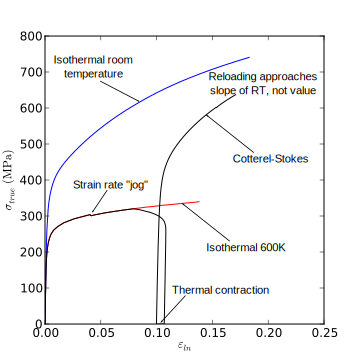
\includegraphics[scale=1.25]{cs_plot.pdf}
\caption{{\small  Results of Cottrell-Stokes simulations with the CP 
model using MTS hardening.} \label{fig:cv-test}}
%
\end{center}
\end{figure}
%


\noi \ul{Stage IV Hardening Generates Approximate Size Effects}

\noi Input files in the \ttt{size\_effect} subdirectory of  directory  \ttt{example\_problems\_cp}
demonstrate non-homogenized CPFEM models
and the geometric Stage IV hardening option. These two models
are identical cubes of cubic grains, where the only difference
is the grain size.  With a non-gradient-enhanced model, the responses
are identical during deformation in tension. However, the gradient Stage IV hardening
introduces a size-effect, where the model with smaller grain sizes (and hence
steeper grain gradients) shows more hardening (increases of some
stress components) than the model with larger grains.
This can be viewed as a physical Hall-Petch-type effect. 

\noi \ul{Use of CP model in MPI-Based Parallel Analyses}

\noi The model in the \ttt{mpi\_restart} subdirectory of  directory  \ttt{example\_problems\_cp}
demonstrates running
the crystal plasticity model in parallel with MPI domain decomposition.  It also
demonstrates that the restart capability of WARP3D with the CP material,
including restarts of un-homogenized models where the angles are input
from a separate flat file.

\noi \ul{Use of Simple Voce Hardening}

\noi The model in the \ttt{simple\_voce} subdirectory of  directory  \ttt{example\_problems\_cp}
demonstrates running
the crystal plasticity model with the temperature and rate independent 
Voce hardening. The model is a single element loading in tension.

\bibliographystyle{plainnat}
\bibliography{citations}

\end{document}
